\chapter{Konzept und Implementation}\label{ch:konzept}

Im Folgenden soll auf die in \Cref{ch:grundlagen} beschriebenen Patterns und Grundlagen zurückgegriffen werden und, zusammen mit den in \Cref{ch:analyse} analysierten Komponenten und Navigationswegen, das erstellte Konzept und die dazugehörige Implementation diskutiert werden.

\section{Konzeption einer Ordnerstruktur}

Die Konzeption einer Ordnerstruktur steht zu Beginn der Bearbeitung und Implementation der Applikation und soll für eine allgemeine Verbesserung der Applikationsstruktur gegenüber den in \Cref{ch:einleitung} genannten Strukturproblemen sorgen. Die Struktur ist dabei nach folgendem Regelwerk aufgebaut:

\begin{itemize}
\item Im Root-Verzeichnis des Repositories befinden sich Konfigurationsdateien des Package-Managers Cocoapods, Github-Workflows und weitere Hilfsdateien, die nicht direkt zur Codebasis der App gehören. Außerdem befindet sich an dieser Stelle das Applikationsverzeichnis.
\item In der obersten Applikationsebene befinden sich die komponentenspezifischen Ordner nach TLA, sowie die Applikationsklasse selbst und global konfigurierende Codefragmente und Artefakte (z.B. Lokalisierungsdateien, Info.plist).
\item Außerdem in der obersten Applikationsebene befindet sich ein Ordner \texttt{Resources}, in dem sich die Assets (z.B. AppIcon, UI-Elemente), jedoch auch Fonts, Lizenzen, eventuelle HTML-Templates oder andere Datenfragmente befinden.
\item Jede Komponente ist entweder separiert in weitere Teilkomponenten, oder besteht aus einer Auswahl aus den Unterordnern \texttt{Mocks}, \texttt{Views}, \texttt{ViewModels} oder anderen, Backend-Funktionalitäten kapselnden Ordnern.
\item Jedes \texttt{Mocks} Verzeichnis dient zur Bereitstellung von Mock-Objekten für die SwiftUI-Previews.
\item Jedes \texttt{ViewModels} Verzeichnis dient zur Bereitstellung von Modellen, die selbst nicht als Model Teil des Couchbase-Frameworks sind, sondern zusätzlich von Views zur Darstellung benötigt werden.
\item Jedes \texttt{Views} Verzeichnis beinhaltet die Ansichten der Komponente, die zur Darstellung der Applikation benötigt werden.
\end{itemize}

Die Applikation ist somit auf oberster Ebene vertikal geteilt, um eine bestmögliche funktionelle Separation der Module voneinander zu bestärken. Auf Komponenten-Ebene ist die Applikation horizontal geteilt, um die Ansichten bestmöglich von Datenmodellen und den dazugehörigen Backend-Funktionalitäten zu trennen. Außerdem soll darauf geachtet werden, dass die Klassen und Dateien innerhalb der jeweiligen Module möglichst als Präfix den Modulnamen tragen, beispielsweise \texttt{TwitterHTMLView} der Komponente Twitter, um sie später im Code besser voneinander unterscheiden und separieren zu können.

\section{Einführung eines Copyright-Templates}

Standardmäßig ergänzt XCode (iOS-IDE von Apple) beim Erstellen einer leeren Codedatei immer einen Copyright-Hinweis. Dieser ist jedoch nicht immer deskriptiv genug bzw. referenziert die dem Projekt beigefügte Lizenz nicht korrekt. Außerdem enthält der Copyright-Hinweis standardmäßig den gewählten Dateinamen, wodurch bei einer späteren Modifikation des Dateinamens auch immer gleichzeitig der Hinweis modifiziert werden muss, um Diskrepanzen zwischen dem Dateinamen und dem Hinweis zu verhindern. Deshalb wurde im Rahmen des Projektes ein Copyright-Template erstellt und in XCode, auf alle Entwickler des Projektes übergreifend, eingebunden.

\begin{figure}[H]
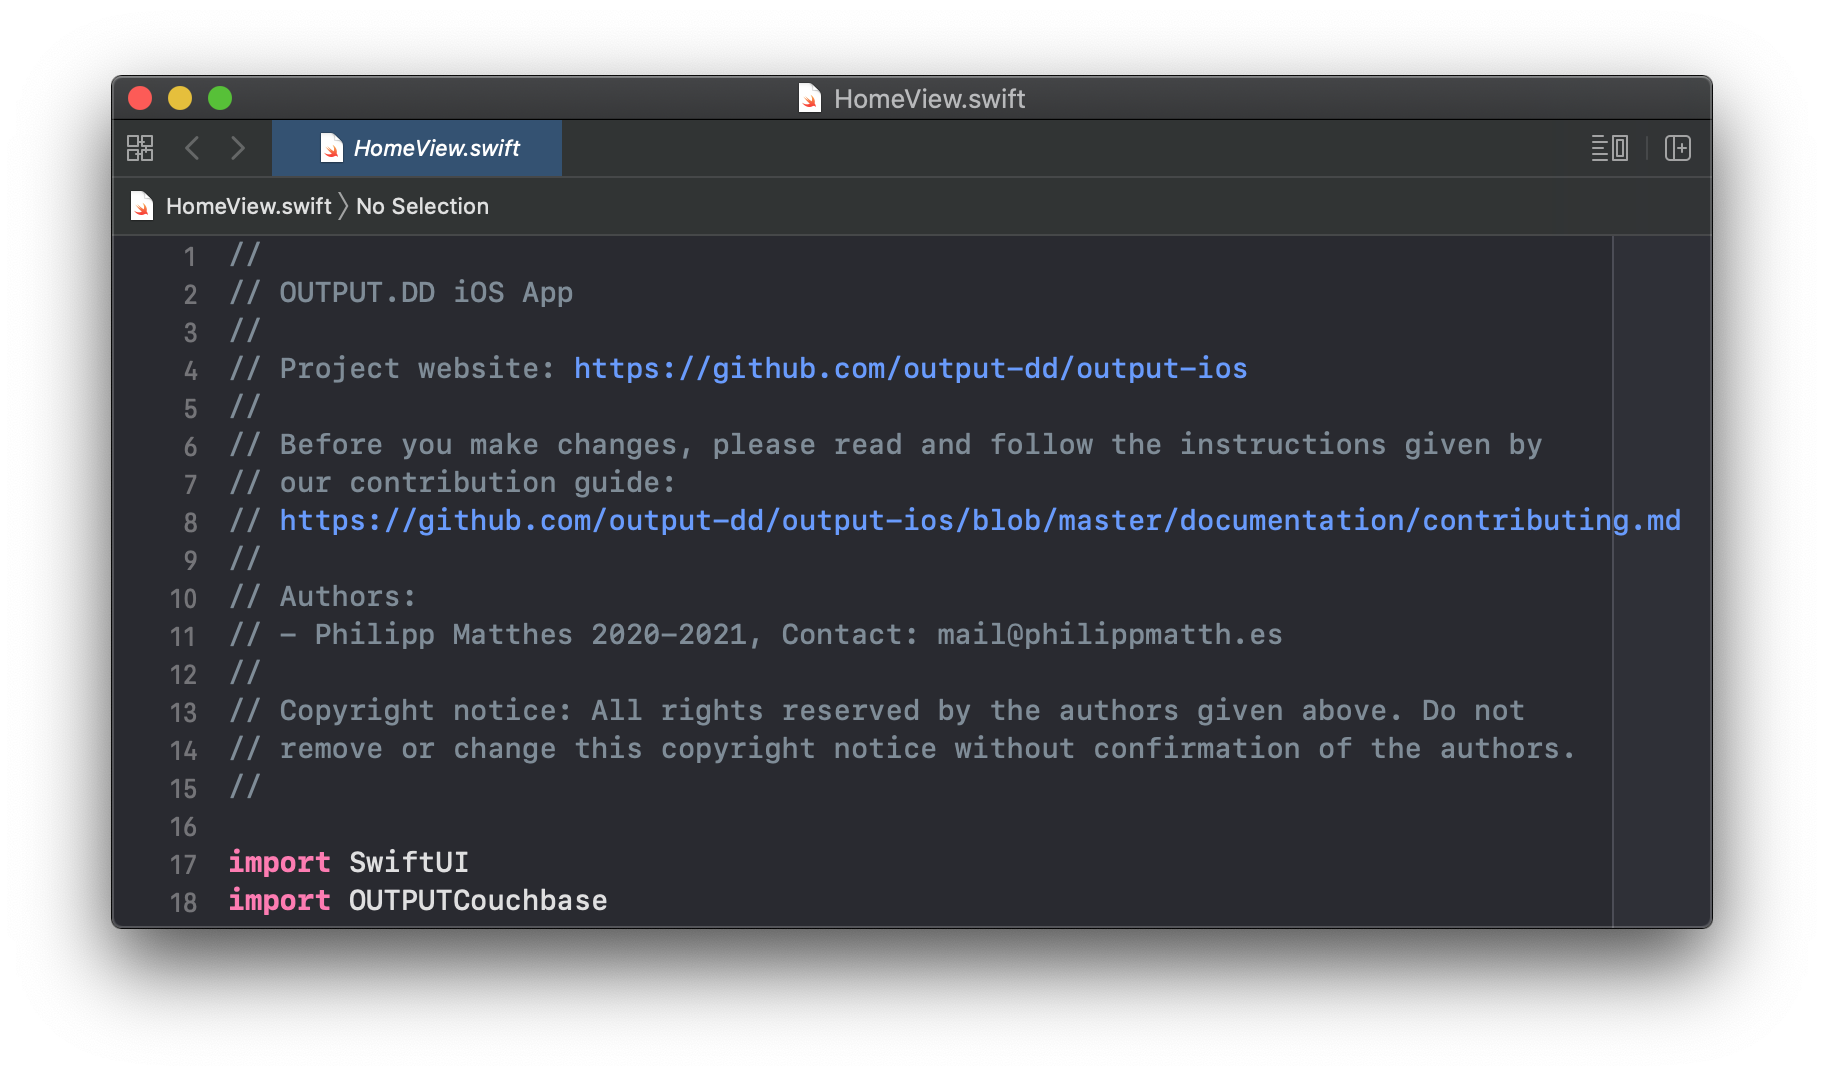
\includegraphics[width=\linewidth]{copyright.png}
\caption{Die erstellte Copyright-Template am Beispiel der HomeView.}\label{fig:copyright}
\end{figure}

Wie in \Cref{fig:copyright} sichtbar, enthält die Copyright-Template zusätzlich zu Hinweisen und Links über die Herkunft des Code-Fragmentes auch einen Link zu den Contribution-Guidelines, welche später im Konzept erläutert werden. Die Template ist bewusst so ausgelegt, dass sich mehrere Autoren inklusive ihrer Kontaktinformationen eintragen können. Letzteres ist wichtig, da sich im Projektteam noch nicht auf eine Lizenzierung der App unter einer Open-Source-Lizenz festgelegt wurde und daher die Codefragmente unter das Kopierrecht des Autors fallen. Sollte eine Weiterverwendung der Codefragmetes über den ursprünglich dafür bestimmten Rahmen stattfinden, so können die Autoren hierüber kontaktiert werden.

\section{Einführung von Codierungsrichtlinien}

Um das zusätzlich in der bestehenden Applikation identifizierte Problem mit der allgemeinen Degradation der Codequalität zu mitigieren und dieser präventiv entgegen zu wirken, wurde als statisches Codeanalysetool SwiftLint eingeführt und konfiguriert.

\begin{figure}[H]
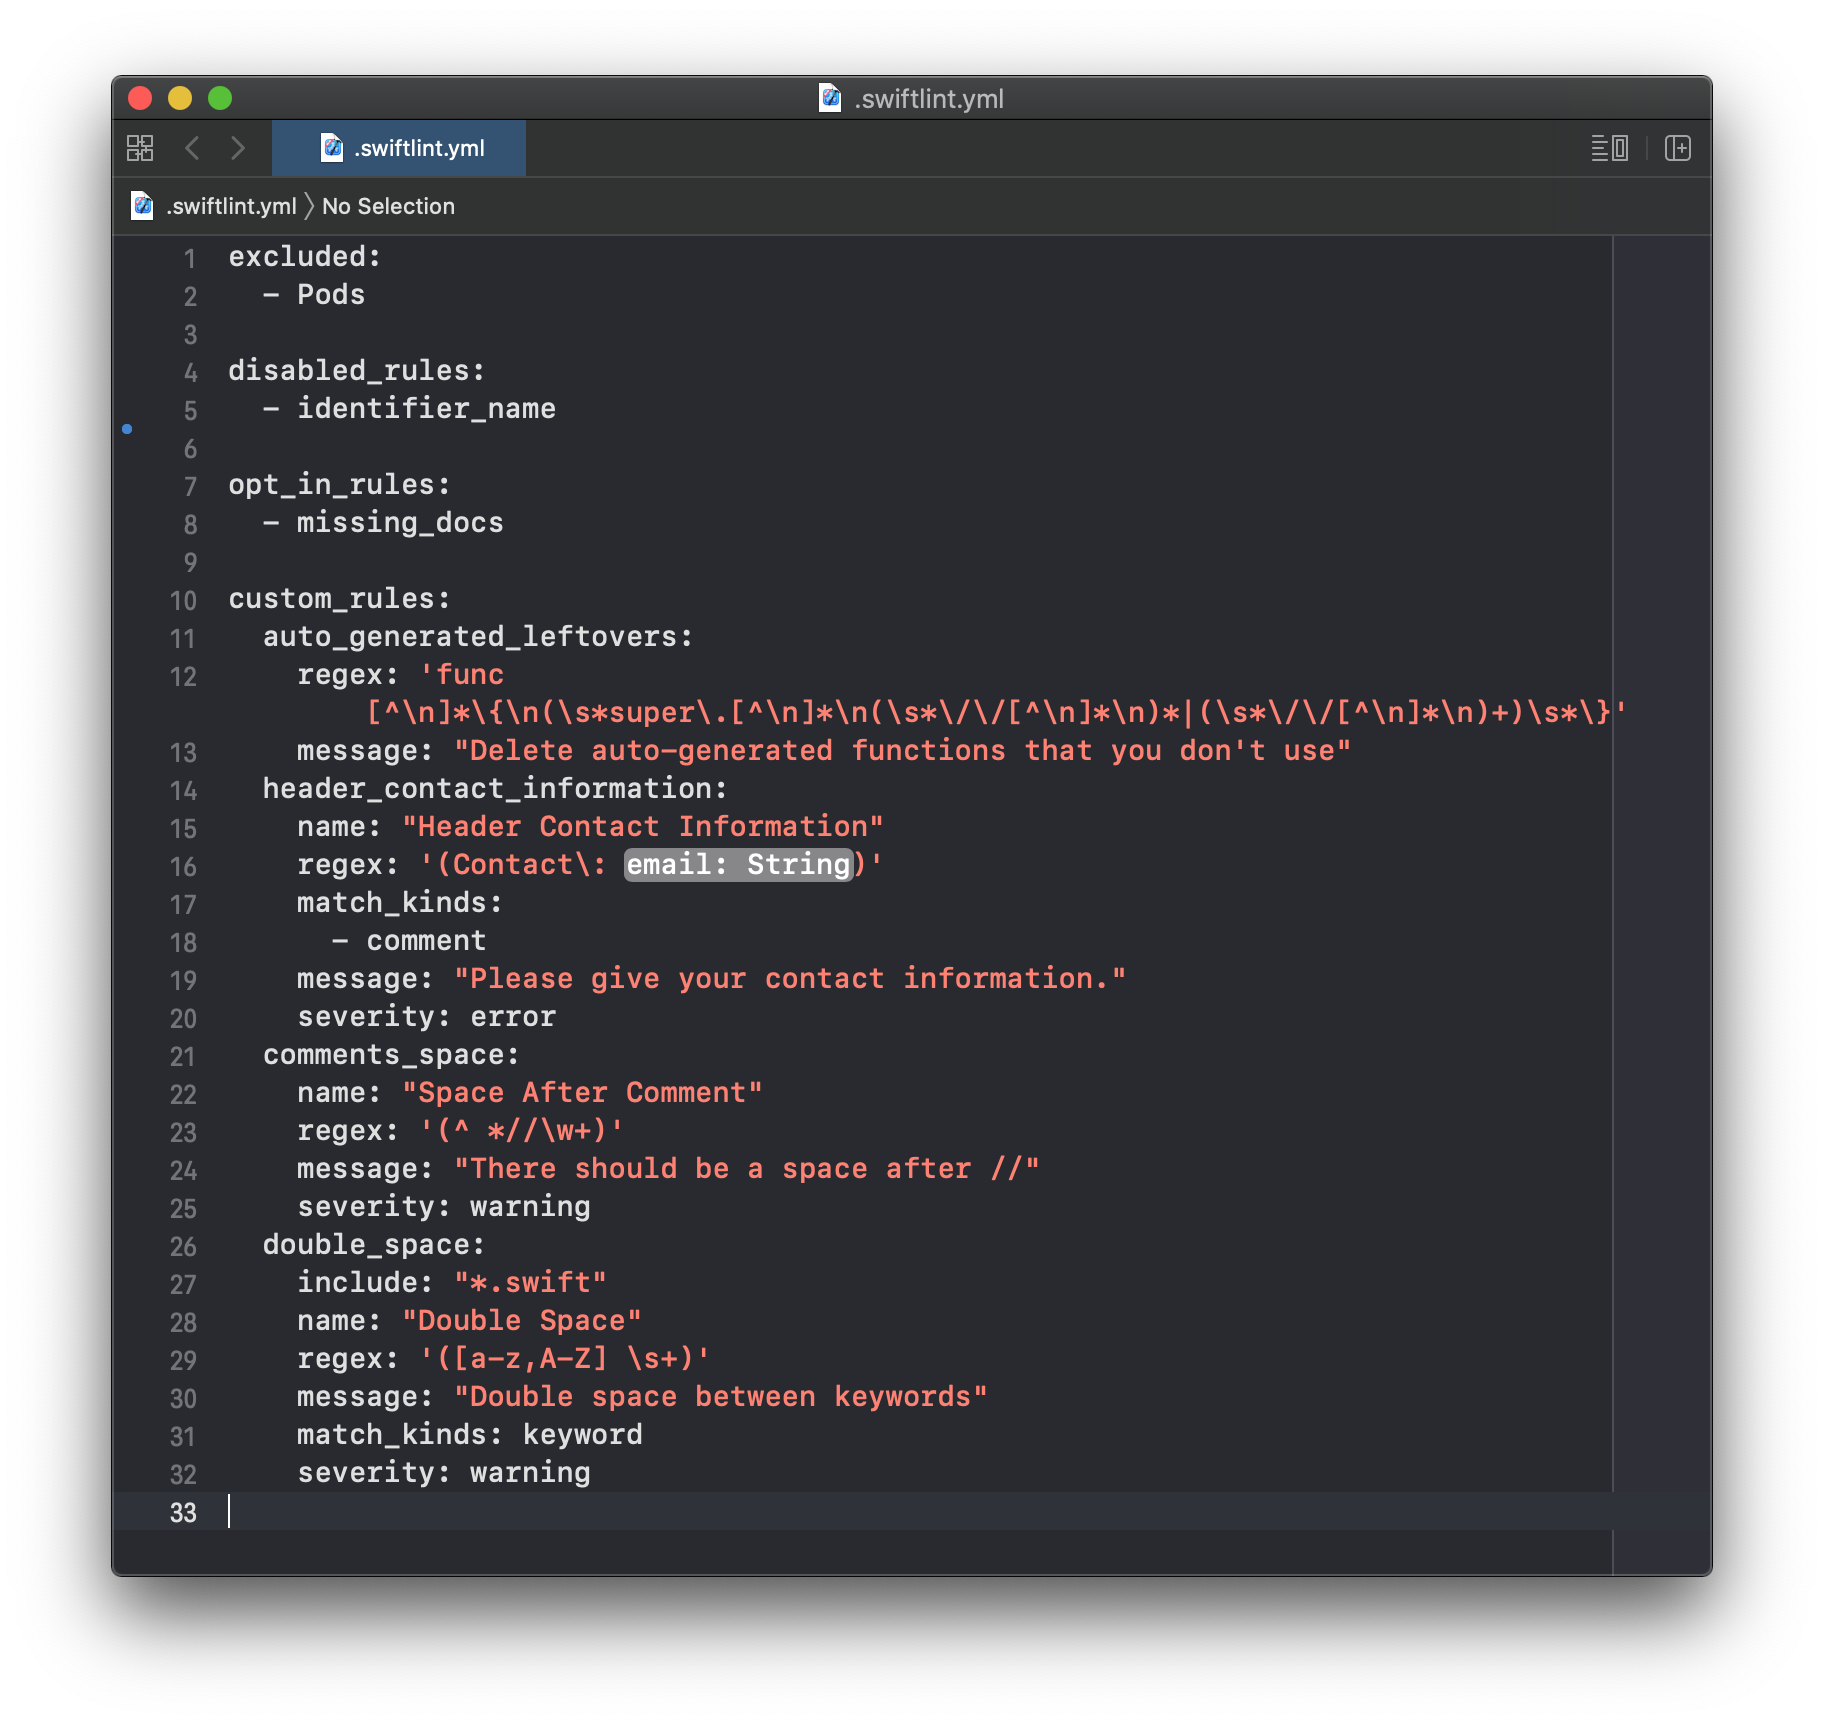
\includegraphics[width=\linewidth]{swiftlint.png}
\caption{Die Konfiguration des statischen Codeanalysetools SwiftLint.}\label{fig:swiftlint}
\end{figure}

In \Cref{fig:swiftlint} ist die Konfiguration von SwiftLint gezeigt. Neben gewöhnlichen Konfigurationen des Frameworks beinhaltet die Konfiguration auch eigene Regeln, darunter eine Regel, die auf das Vorhandensein des Copyright-Templates prüft. Das Tool wurde anschließend im Buildprozess von XCode integriert, so dass bei einer Verletzung der Codierungsrichtlinien diese innerhalb des Editors als Warnung (oder bei schwerwiegenden Verletzungen als Error) markiert wird und refaktorisiert werden kann.

\section{Implementation des Frontends}

Nach der Konzeption einer klaren Ordnerstruktur, sowie der Vorbereitung der Implementation mithilfe der Einführung des Copyright-Templates und der Installation eines statischen Code-Checkers wurde mit der Implementation des Frontends begonnen. Die Implementation fand hierbei entkoppelt vom Datenbank-Backend statt, indem für jede Ansicht temporäre ViewModels entworfen wurden, die zur Darstellung benutzt werden konnten. Dies ergab wesentliche Vorteile im Entwicklungsprozess:

\begin{itemize}
\item Die Ansichten konnten schnell mithilfe der SwiftUI-Preview erstellt werden, ohne eine aufwändige Anbindung des Datenbank-Backends oder eine entsprechende Daten-Initialisierung.
\item Die Ansichten konnten durch diesen Zwischenschritt leichter vom Datenbank-Backend separiert werden.
\end{itemize}

Außerdem konnte auf diese Weise in wenigen Wochen ein voll funktionsfähiges UI erstellt werden, lediglich mit einer fehlenden Anbindung an das Datenbank-Backend. Das UI konnte so bereits getestet und zwischen der iOS- und der Android-Version abgeglichen werden.

\begin{figure}[H]
\includegraphics[width=\linewidth, bb=0 0 2297 2000]{ui.pdf}
\caption{Die Hauptansichten des UI der neu implementierten App im Profil.}\label{fig:ui}
\end{figure}

In \Cref{fig:ui} werden die 5 Hauptansichten der App gezeigt, außerdem wurden noch einige weitere Ansichten (analog zur Dialoglandkarte) implementiert. Alle Ansichten orientieren sich hierbei am Aufbau der bisherigen Ansichten in der bestehenden App. Gleichzeitig wird das UI an vielen Stellen modernisiert, modularisiert und nutzerfreundlicher gestaltet. Zur Modernisierung gehört bspw. eine Implementation eines Dark-Mode Features, welches sich an der Systemeinstellung des Nutzers orientiert und bei Dunkelheit die Augen vor zu viel Helligkeit schützt. Außerdem wurden an verschiedenen Stellen bestimmte Animationen implementiert, bspw. bei dem Berühren eines Buttons, um die Benutzung der UI noch intuitiver und zufriedenstellender zu gestalten. Gleichzeitig wurde insbesondere auch auf Grundprinzipien des Usability Engineerings geachtet, sodass Buttons immer eine bestimmte Größe je nach Platzierung im UI besitzen und die meisten Interaktionen in der App in der unteren Hälfte des Bildschirms mit dem rechten Daumen getätigt werden können. Bei wichtigen Interaktionen erhält der Nutzer zudem ein haptisches Feedback. Zur Modularisierung des UI tragen bestimmte UI-Komponenten bei, die innerhalb verschiedener Ansichten mehrfach wiederverwendet werden können, wie eine (auch in \Cref{fig:ui} sichtbare) CardView oder ein eigener ViewPaginator. Nicht nur bei letzterem, sondern auch bei der Auswahl der Formen, Farben und Fonts wurde auf die Vorgaben aus der OUTPUD.DD Corporate Identity geachtet, so dass beispielsweise die Farbpalette übernommen wurde und ein wiederverwendbarer ViewModifier für die Applizierung des OpenSans-Fonts innerhalb von SwiftUI implementiert wurde. Außerdem wurde die Applikation vollständig internationalisiert, auf Grundlage der von SwiftUI bereitgestellten Funktion zur String Interpolation in Localizable.strings Dateien.

\paragraph{Reimplementation von weiteren Teilansichten: } Zusätzlich zu einer Reimplementation des gesamten UI, inklusive komplexerer Ansichten wie die Reward-Ansicht mit einer Konfetti-Animation, wurde in der Map-Ansicht das Google Maps Framework durch das MapBox Framework ersetzt. Vor dieser Entscheidung wurde anhand einer internen Team-Diskussion abgewägt, welches der beiden Frameworks zukünftig genutzt werden soll. Aufgrund der Nutzerfreundlichkeit, der leichten Anbindbarkeit und der Verwendung des Frameworks in anderen Projekten der Professur entschieden wir uns für MapBox. In der Twitter-Ansicht wurde während der Implementation des Frontends ein weiteres Problem identifiziert, welches darin bestand, dass das von der bestehenden App genutzte Twitter-Framework von Twitter nicht länger unterstützt wurde und damit die Gefahr bestand, dass in Zukunft diese UI-Komponente nicht mehr funktionieren könnte. Daher konzipierten wir als Lösung hierfür eine rein auf HTML basierende TwitterHTMLView, welche das von Twitter bereitgestellte Twitter Widget nutzt. Dies hat nicht nur den Vorteil, dass das nicht mehr unterstützte Framework entfernt werden konnte, sondern auch, dass kein API-Schlüssel mehr für die Verwendung notwendig ist.

\section{Integration einer CI-Pipeline}

Um die Applikation an verschiedene Tester über die von Apple bereitgestellte App \enquote{TestFlight} zu verteilen, bietet XCode die Möglichkeit, die Applikation zu signieren, in einem Archiv zu verpacken, dieses an die Plattform AppStore Connect zu übermitteln, und von dort (unter Vorausfüllung von Testinformationen) an die Tester zu übermitteln. Dieser Prozess ist jedoch sehr zeitaufwändig und dauert, je nach Tageszeit ca. 20-30 Minuten. Daher bat es sich an, die Applikation in einer Continuous-Integration-Pipeline einzubinden, welche diesen Prozess übernimmt. Hierzu wurde ein GitHub-Workflow adaptiert, der bereits für ein anderes iOS-Projekt (\enquote{Peerbridge} Blockchain Messenger) erstellt wurde. Der Workflow nutzt unter anderem das Framework Fastlane, um die Applikation zu archivieren und an die Tester vollautomatisch zu übermitteln. Hierfür sind einige technische Details von Relevanz, beispielsweise das Importieren des Signatur-Zertifikats in die CI-Pipeline, welche jedoch an dieser Stelle nicht weiter erläutert werden sollen. Für die Distribution wurden die technisch notwendigen Schritte in einem Delivery-Guide zusammengefasst, welcher im App-Repository unter \url{https://github.com/output-dd/output-ios/blob/master/documentation/delivery.md} (Zuletzt abgerufen am 31.1.2021) zu finden ist. Aus der Integration des Workflows bildet sich eine signifikante Zeitersparnis bei der Distribution der Applikation an die Tester. Die Applikation muss lediglich vom Entwickler mit einer Versionsnummer getaggt werden und die Bestimmungen von Apple erfüllen. Letztere sind konkret, dass die Build- und Versions-Nummer vor dem Taggen inkrementiert werden muss, sowie, dass die eventuell notwendigen Berechtigungen in der \texttt{Info.plist} Datei beschrieben sind.

\section{Fusion des Frontends mit dem Datenbank-Backend}

Auf Grundlage des implementierten Frontends und der CI-Pipeline konnten nun sukzessiv die einzelnen Komponenten und Ansichten um eine Backend-Persistierung erweitert und damit die übergangsweise genutzten ViewModels an geeigneten Stellen substituiert werden. Hierzu wurde das Datenbank-Backend über den Package-Manager Cocoapods als privates Pod hinzugefügt und die CI-Pipeline um die entsprechende Berechtigung ergänzt, damit diese auf das private Repository zugreifen kann. Anschließend wurden noch kleinere Änderungen am Datenbank-Backend, vor allem der Datenbank-Modelle vorgenommen, welche sich um Laufe der Zeit leicht geändert hatten. Mithilfe dieser Änderungen konnte nun auf Grundlage der in \Cref{ch:grundlagen} beschriebenen Patterns die Integration beginnen. \\

\subsection{Vorbemerkungen für die Darstellung der SwiftUI-Preview}

Wie in \Cref{ch:grundlagen} bereits angemerkt, ist ein zentrales Feature von SwiftUI die schnelle deklarative Erstellung von Ansichten. Dies wird unter anderem ermöglicht durch eine Echtzeit-Preview der Ansicht in XCode.

\begin{figure}[H]
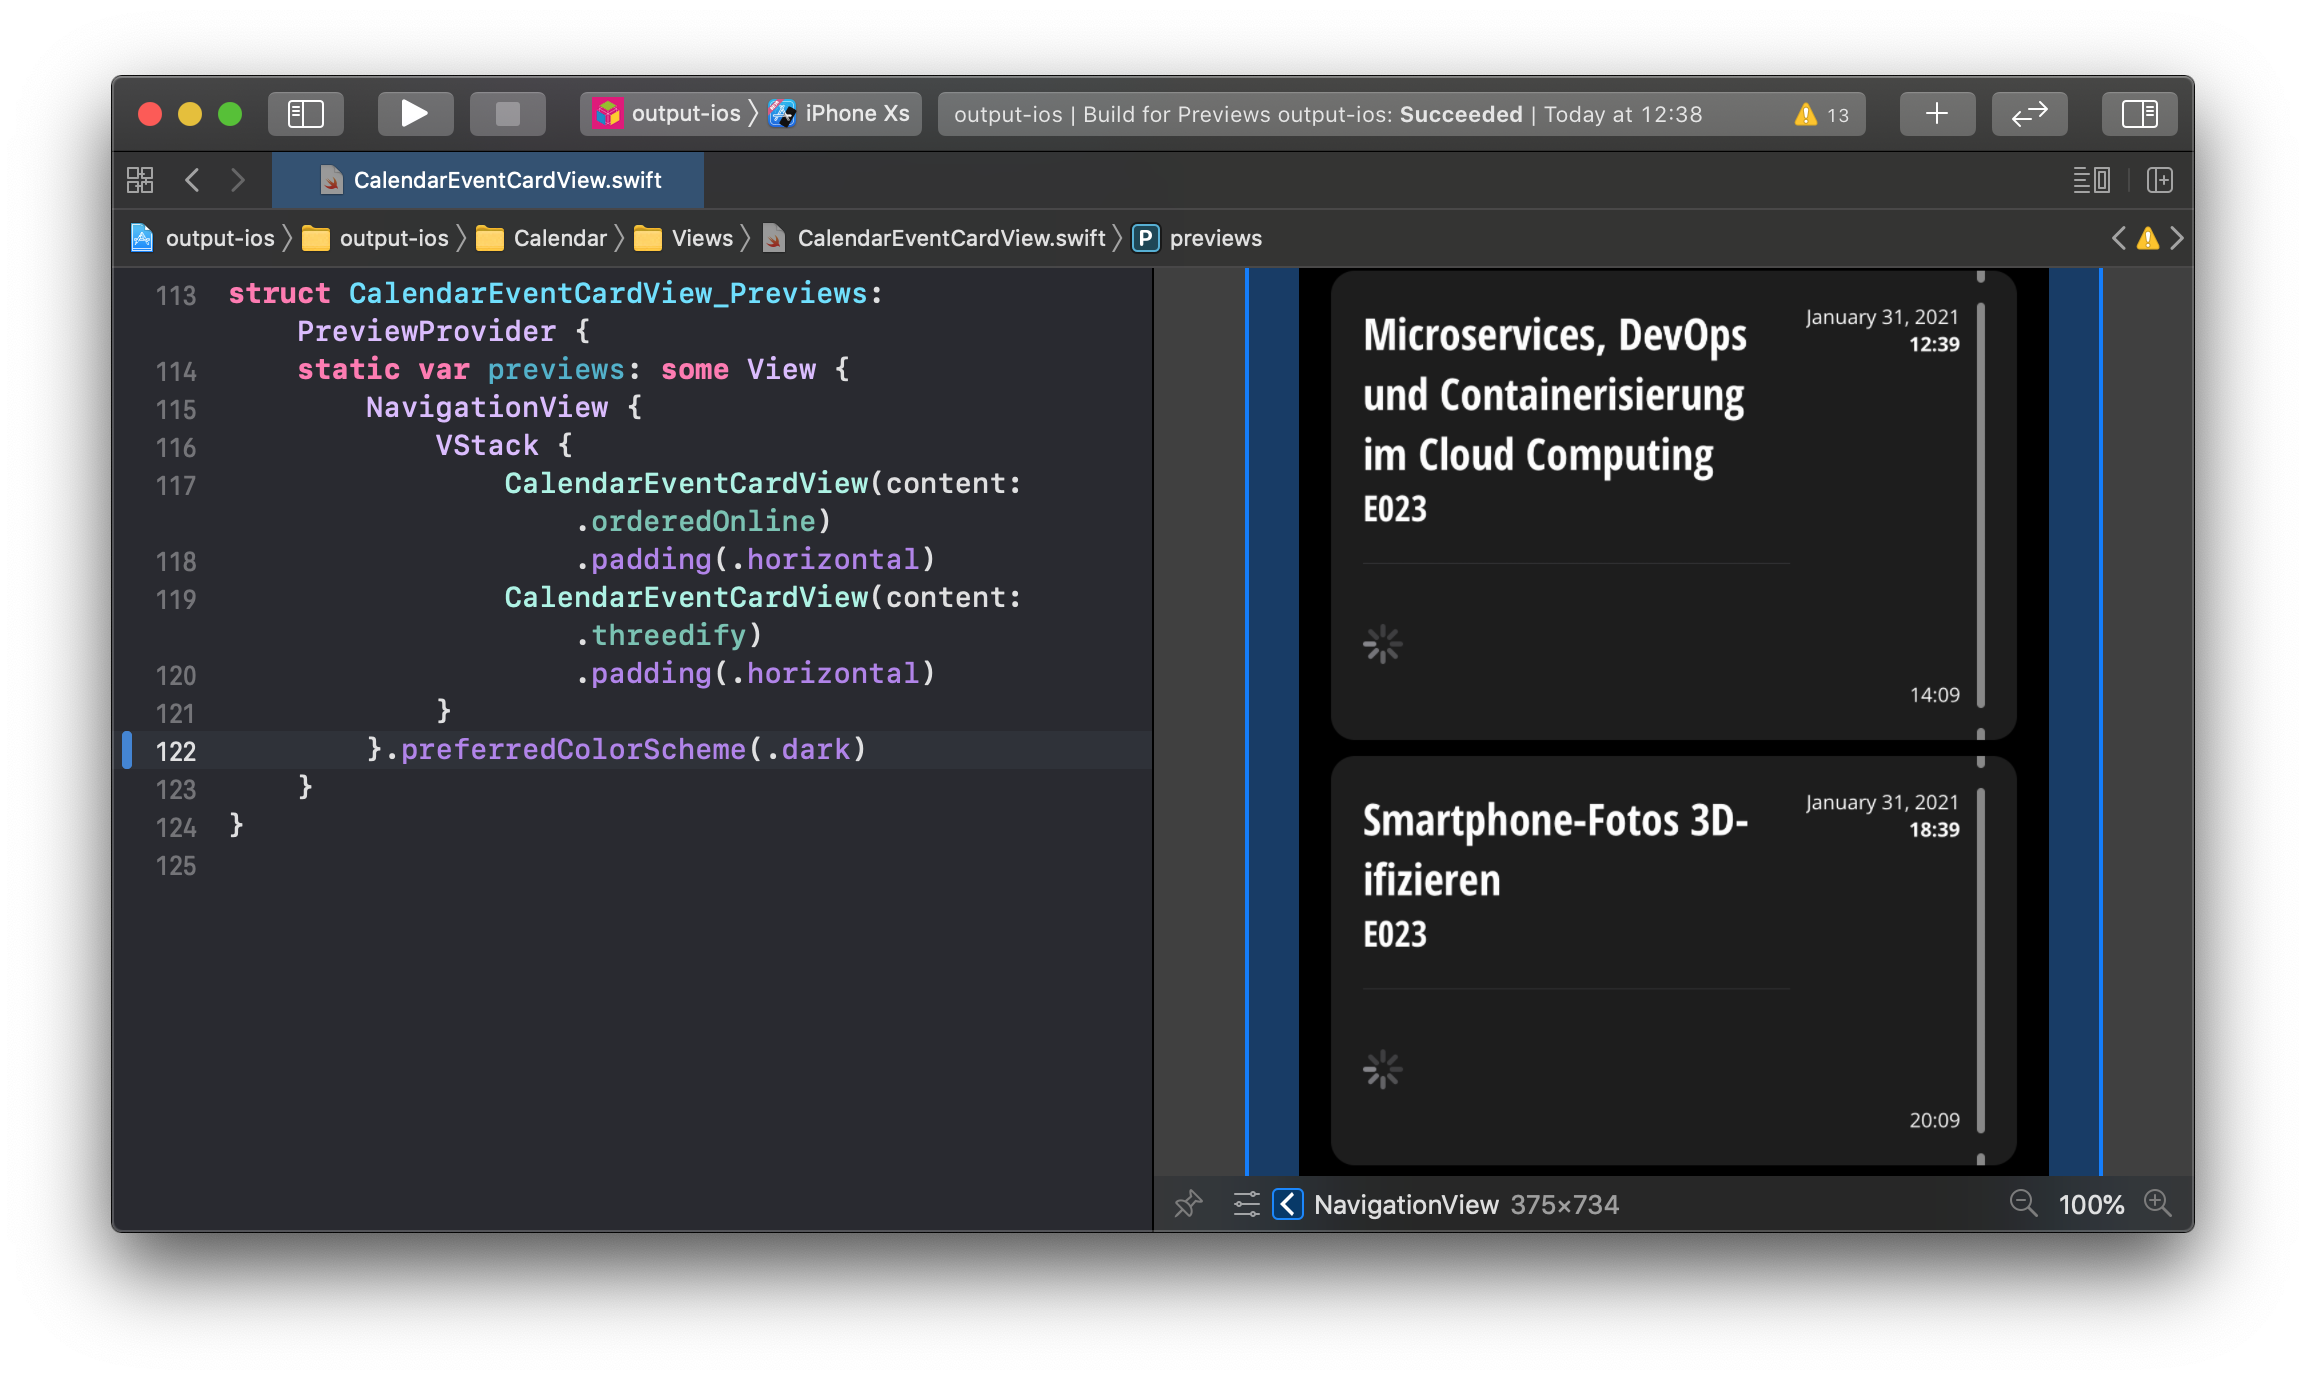
\includegraphics[width=\linewidth]{preview.png}
\caption{Die SwiftUI-Preview der \texttt{CalendarEventCardView} innerhalb von XCode.}\label{fig:preview}
\end{figure}

\Cref{fig:preview} zeigt eine solche Preview innerhalb XCode und wie diese konfiguriert werden kann. Hieraus entwickelt sich jedoch eine weitere Herausforderung bei der Integration des Datenbank-Backends in den Views, denn die Views sollten während der Preview nicht auf ein existierendes Datenbank-Backend angewiesen sein. Eine Vorinitialisierung des Datenbank-Backends in der Preview währe einerseits mit sehr viel zusätzlichem Boilerplate-Code verbunden, andererseits könnte die Preview dann nicht schnell editiert werden, weil bei jeder Änderung der Ansicht das Datenbank-Backend wieder initialisiert werden müsste. Im Folgenden Abschnitt wird die hierfür konzipierte Lösung gezeigt.

\subsection{Nutzung des Environment- und Coordinator-Patterns für die Anbindung der Views}

Um in der Preview der Views auf die zuvor erstellten Mocks zur schnellen Darstellung und Änderung der Ansicht zugreifen zu können und gleichzeitig beim Testen der Applikation auf dem Simulator oder dem physischen Gerät die initialisierte Datenbank zu nutzen, werden die anzubindenden Views mit jeweils einem \texttt{DemoCoordinator} oder einem \texttt{PersistedCoordinator} ausgestattet. Die jeweiligen Koordinatoren erben hierbei von der selben Klasse \texttt{Coordinator} - welche die benötigten Schnittstellen zur Verfügung stellt. Die zwei unterschiedlichen Subklassen-Koordinatoren unterscheiden sich infolge dessen nur darin, ob zum Prozessieren bzw. Holen der Daten die Datenbank genutzt wird, oder lediglich Mock-Objekte für die Preview zurückgegeben werden.

\begin{figure}[H]
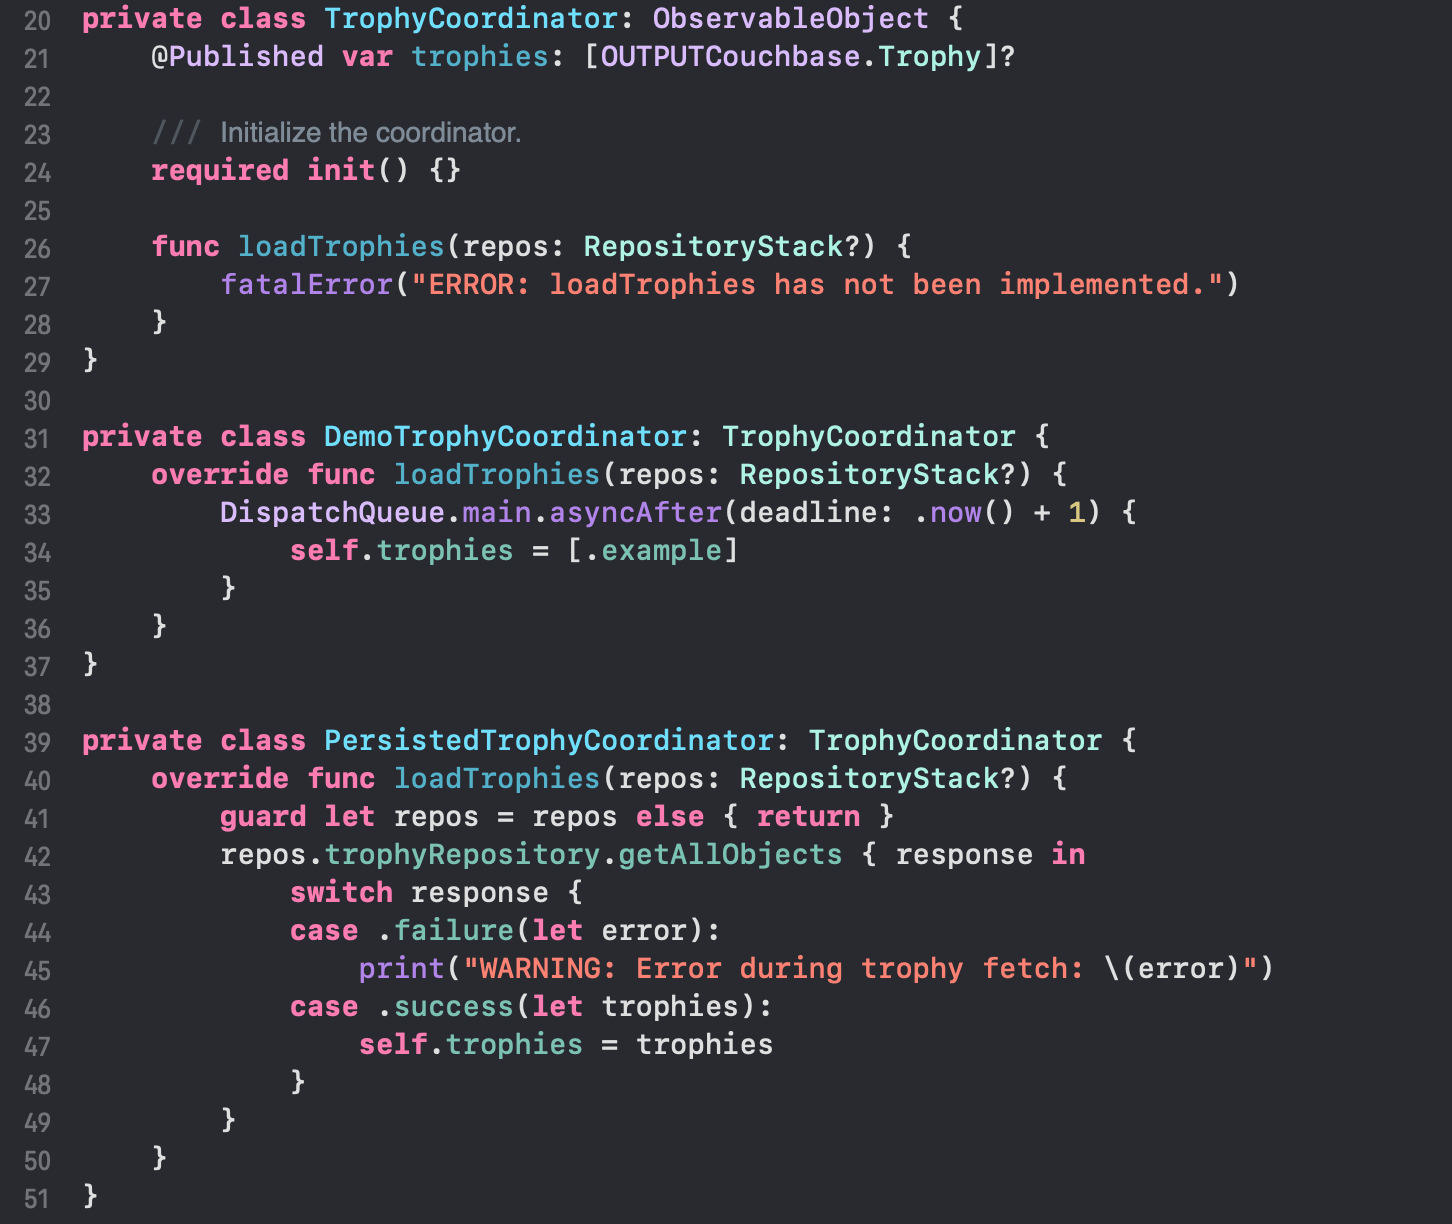
\includegraphics[width=\linewidth]{demo-persisted.png}
\caption{Das Coordinator-Pattern angewandt am Beispiel der Spiel-Trophäen, um eine schnelle SwiftUI-Preview ohne Daten-Initialisierung zu gewährleisten.}\label{fig:demo-persisted}
\end{figure}

Zur Illustration ist dieses Pattern beispielhaft in \Cref{fig:demo-persisted} an der Implementation gezeigt. Der \texttt{TrophyCoordinator} gibt die Schnittstellen vor, an dieser Stelle die geladenen Trophäen (bidirektional referenzierbar durch die Ansicht) sowie eine Funktion zum Laden der Trophäen. Der \texttt{DemoTrophyCoordinator} lädt lediglich gemockte Beispiel-Trophäen nach einer kurzen Verzögerung, um den Ladeprozess zu simulieren. Der \texttt{PersistedTrophyCoordinator} greift auf die Repositories und damit auf die Datenbank zu, um die tatsächlich persistierten Trophäen zu laden.

\begin{figure}[H]
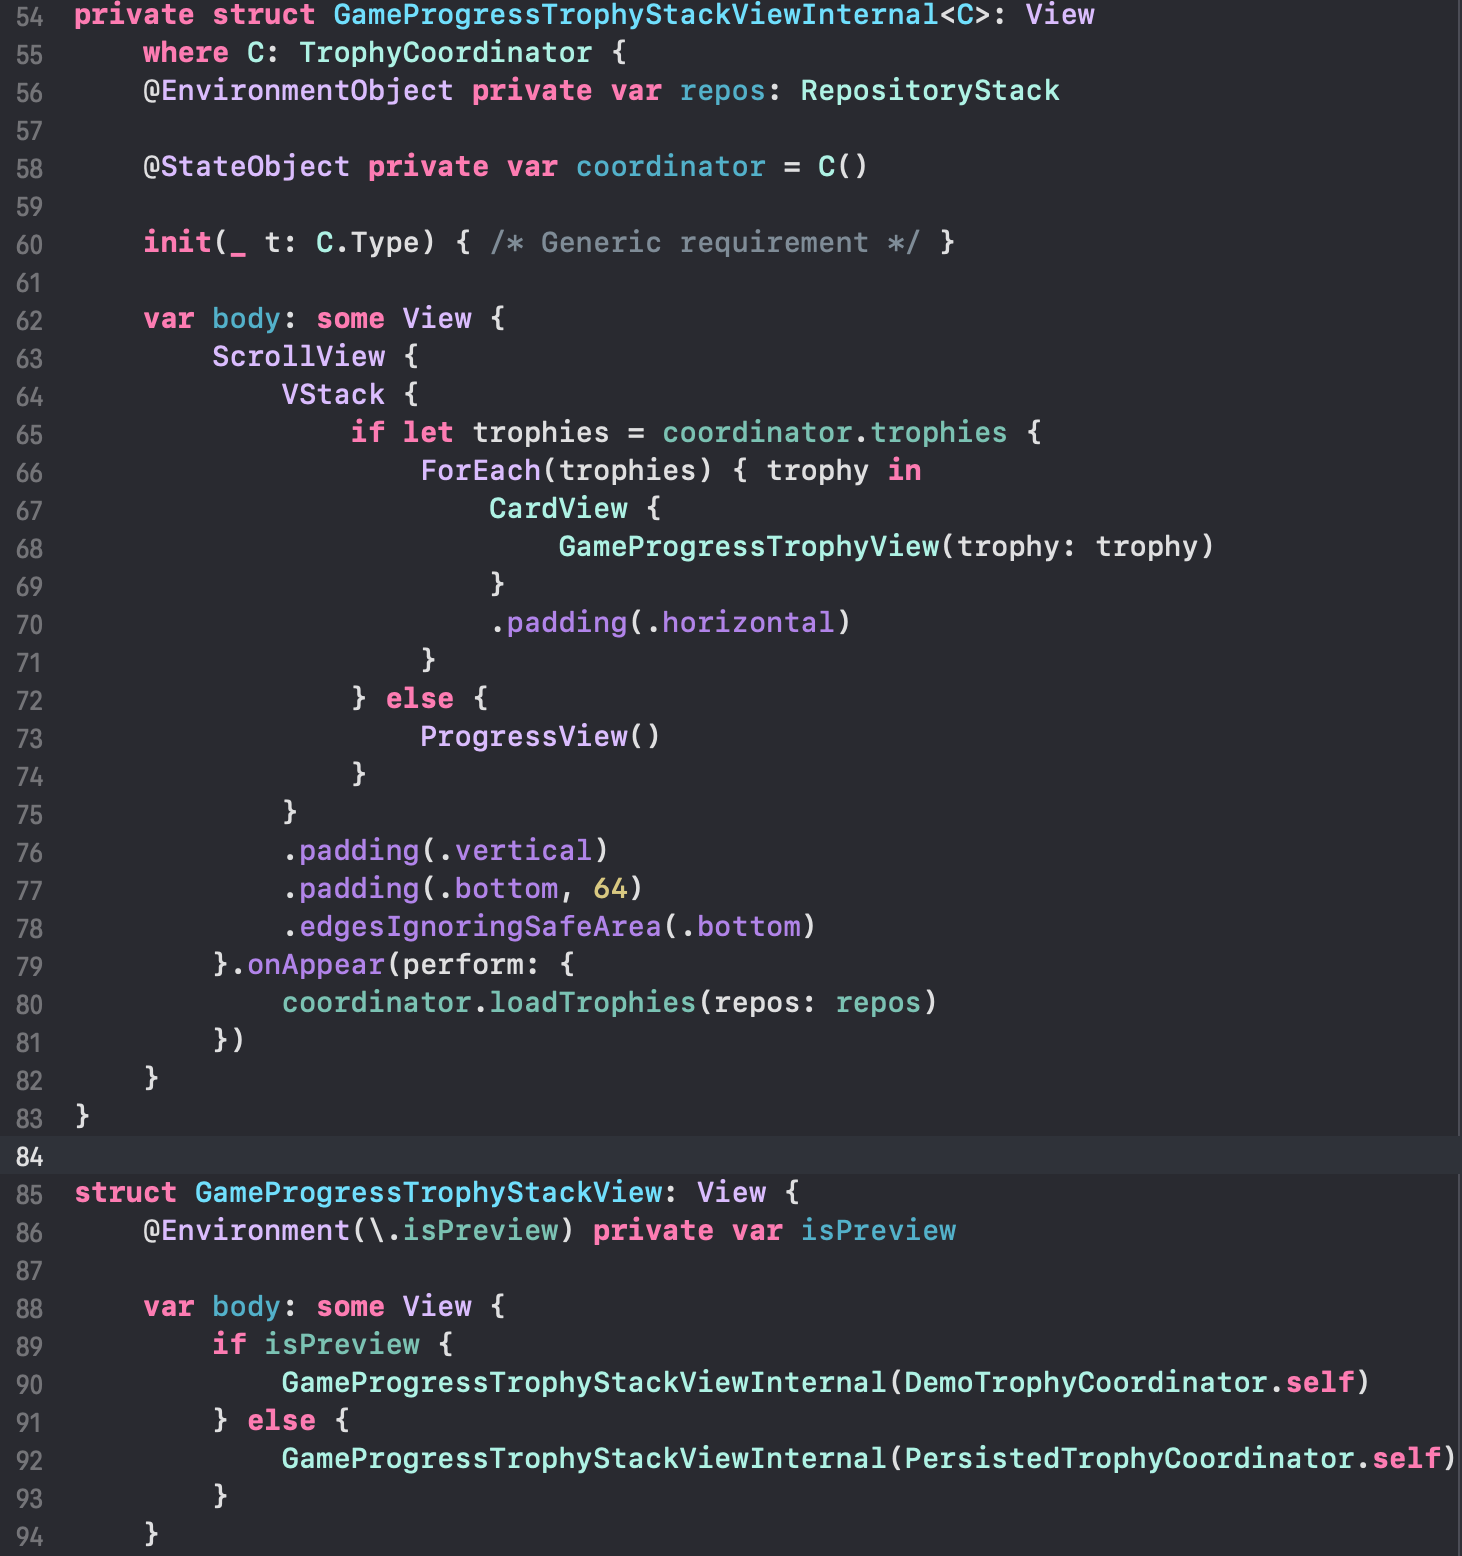
\includegraphics[width=\linewidth]{demo-persisted-view.png}
\caption{Die Anbindung der Koordinatoren an die View im Beispiel der \texttt{GameProgressTrophyStackView}.}\label{fig:demo-persisted-view}
\end{figure}

Die Integration der Koordinatoren erfolgt über die Übergabe als generischen Typparameter im Konstruktor der View. Um die Koordinatoren außerhalb der View-Code-Datei unsichtbar zu machen und nicht den globalen Scope zu verschmutzen, in dem die Koordinatoren keine Bedeutung haben (da sie sich nur auf die einzelne View beziehen) wird die Entscheidung, welcher Koordinator genutzt wird, durch ein Umgebungsattribut \texttt{isPreview} inferiert. Dieses Umgebungsattribut wird aus der Prozessumgebung bezogen, welche Informationen beinhaltet, ob es sich bei der aktuellen Ausführung um eine SwiftUI-Preview-Umgebung handelt, oder nicht. Entsprechend wird der \texttt{DemoCoordinator} nur genutzt, wenn es sich um eine SwiftUI-Preview-Umgebung handelt. Dieses Pattern wurde auf alle Views angewandt, welche bei der Ausführung auf dem Gerät (physisch oder Simulator) mit der Datenbank kommunizieren.

\subsection{Nutzung des Proxy-Patterns für die Initialisierung der Datenbank}

Um die Datenbank zu initialisieren, wird auf das in \Cref{ch:grundlagen} erläuterte Proxy-Pattern zurückgegriffen.

\begin{figure}[H]
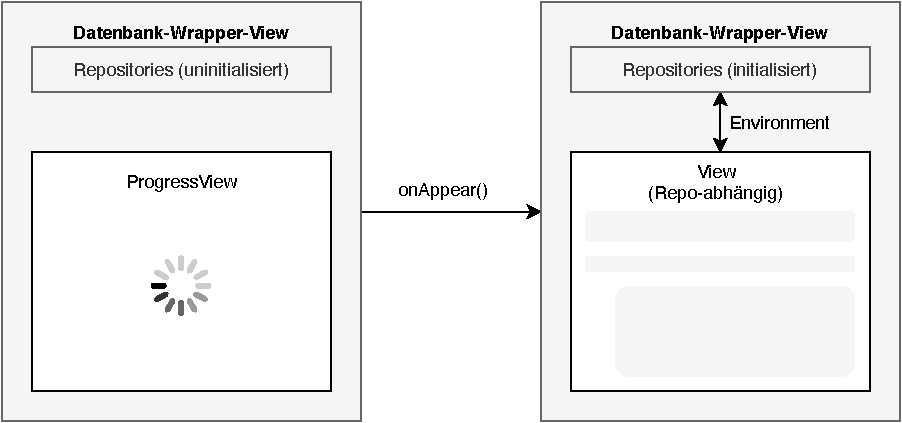
\includegraphics[width=\linewidth, bb=0 0 432 203]{proxy.pdf}
\caption{Abstrakte Übersicht über die Initialisierung der Datenbank.}\label{fig:proxy}
\end{figure}

\Cref{fig:proxy} zeigt die Initialisierung der Datenbank. Hierzu werden die datenbankabhängigen Ansichten als innere View mitgegeben. Sobald nun die Gesamtansicht erscheint (in diesem Fall beim Start der App) wird zunächst ein Loading-Indicator angezeigt und die Datenbank initial erstellt bzw. geladen. Anschließend werden die Repositories auf der Datenbank initialisiert und über das Environment der Ansicht an die Unteransichten übergeben. Die Unteransichten besitzen hierdurch die Möglichkeit, über die Umgebung auf die Repositories und somit auch auf die persistierten Objekte zuzugreifen.

\subsection{Validierung der Datenbankfunktionalität}

Um die Anbindung der Datenbank zu validieren, wurden im Rahmen der Implementation zu Testzwecken auch mehrere Daten-Initialisierer implementiert. Unter anderem wurden hierzu auch Test-Skripte entwickelt, bspw. um die Heatmap zu generieren. Somit konnte für die angebundenen Ansichten sichergestellt werden, dass unter Existenz von Objekten in der Datenbank diese korrekt behandelt und dargestellt werden. Gleichzeitig konnte auch die Performanz der Applikation getestet werden, beispielsweise durch die Generierung von mehreren tausenden Einträgen im Leaderboard der Gamification.

\subsection{Anbindung der Synchronisationskomponente}



\subsection{Validierung der Synchronisation}

\subsection{Listener- und Eventbasierte Anbindung der Gamification}

\subsection{Integration des Crowd-Monitoring-Frameworks}
